\chapter{Metodo Proposto}
Il metodo che ha fornito i migliori risultati, sia per il task di classificazione che per quello di regressione, è stato ottenuto affinando le diverse strategie sperimentate sopra elencate. Esso sfrutta ancora una volta l’architettura di rete VGG16 pre-addestrata sul dataset “ImageNet” e si basa essenzialmente sull’aggiunta di “data augmentation”, ovvero una tecnica che permette di aumentare i dati in maniera sintetica trasformando “al volo” i dati in input in maniera casuale e facendo in modo che, dopo la trasformazione, l’etichetta sia ancora valida, e su un opportuno “fine-tuning” della reta.\\
Ciò ci ha permesso di ottenere un modello più robusto e capace di generalizzare, riducendo l’overfitting.
Le trasformazioni, applicate solo in fase di training, sono le seguenti:
\begin{itemize}
	\item[•]Random Horizontal Flip: flip orizzontale random con probabilità 0.5
	\item[•]Color Jitter: il valore di ogni pixel viene perturbato leggermente in maniera casuale
	\item[•]Random Rotation(20): rotazione random dell’immagine tra -20° e +20°
	\item[•]Random Crop(128): crop 128x128 viene estratto casualmente dall’immagine
\end{itemize}
Per compatibilità, in fase di test vengono estratti crop 128x128 dalla parte centrale dell’immagine.
A seguito delle trasformazioni, siamo costretti ad adattare la struttura dell’architettura per accettare in input immagini da 128x128, andando essenzialmente a modificare i livelli lineari del blocco fully connected.
\\ \\
E’ stato effettuato poi il fine-tuning del modello, freezando tutti i livelli del modulo “features” che contiene i blocchi convoluzionali, ad eccezione degli ultimi due blocchi, e del blocco fully connected del modulo “classifier”. \\
In questo modo verranno aggiornati solamente i parametri dei livelli del blocco fully connected, ed i parametri dei livelli degli ultimi due blocchi convoluzionali. \\
Sono stati poi cambiati i dropout nei livelli fully connected, impostando come probabilità 0.25.

\section{Classificazione}
\begin{figure}[H]
	\centering
	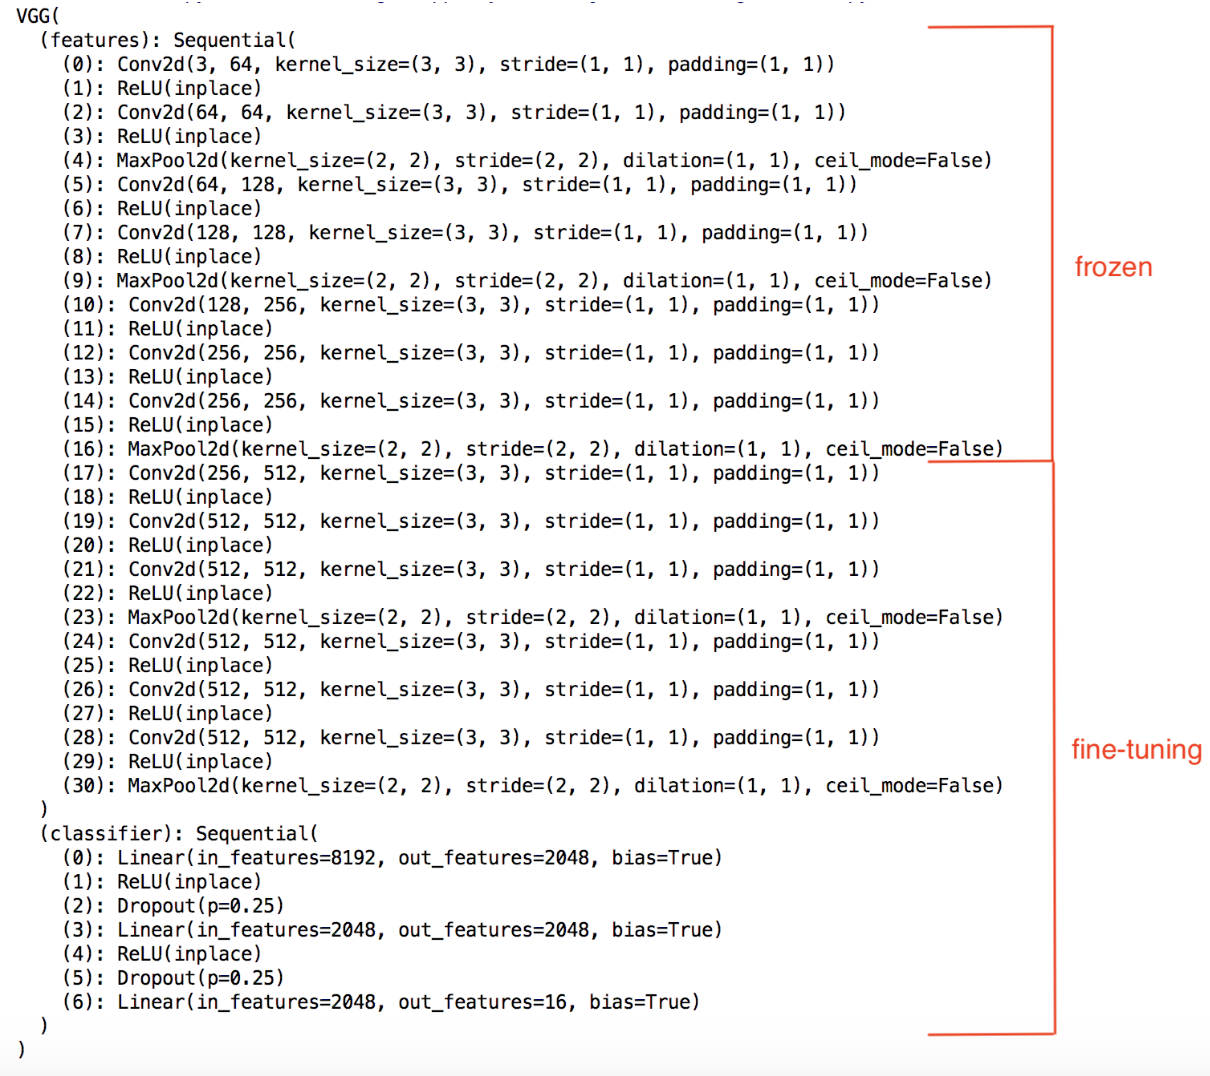
\includegraphics[scale=0.70]{image29.png}
\end{figure}
Poichè il task di classificazione richiede in output 16 classi, sono stati modificati gli ultimi livelli lineari impostando a 16 le features di output dell’ultimo livello con classificatore softmax.
Per la procedura di training utilizziamo: 
\begin{itemize}
	\item[•]Learning rate: 0.00001
	\item[•]Momentum: 0.9
	\item[•]Weight decay: 0.000001
\end{itemize}
Come loss function utilizziamo cross entropy loss, come funzione di attivazione utilizziamo ReLU, mentre come metodo di learning utilizziamo SGD. \\
Abbiamo allenato il modello per 400 epoche, ed abbiamo ottenuto i seguenti risultati:

\subsection{Accuracy}
\begin{figure}[H]
	\centering
	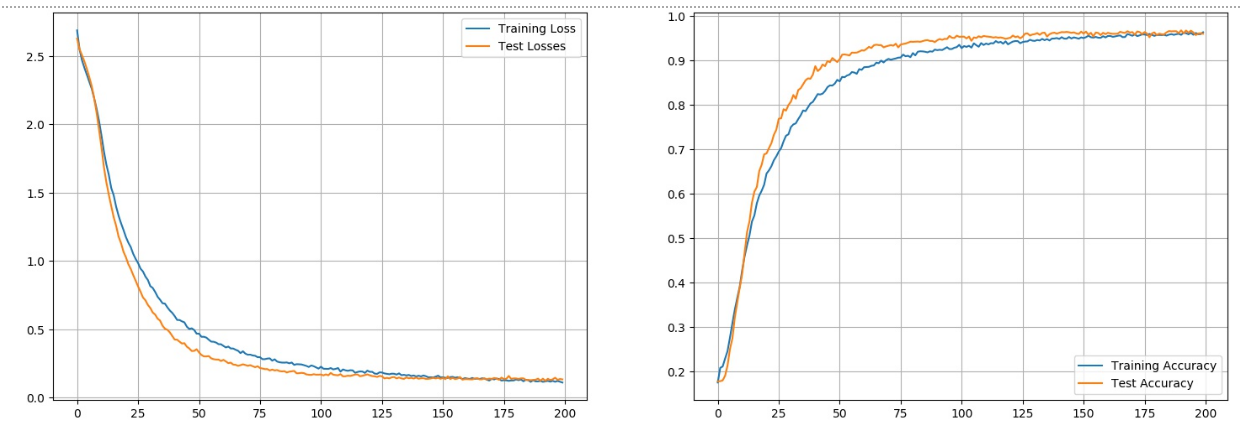
\includegraphics[scale=0.65]{image30.png}
\end{figure}
Dai due plot, di cui sopra, possiamo osservare la convergenza della validation/training loss e della validation/training accuracy.

\subsection{Matrice di confusione}
\begin{figure}[H]
	\centering
	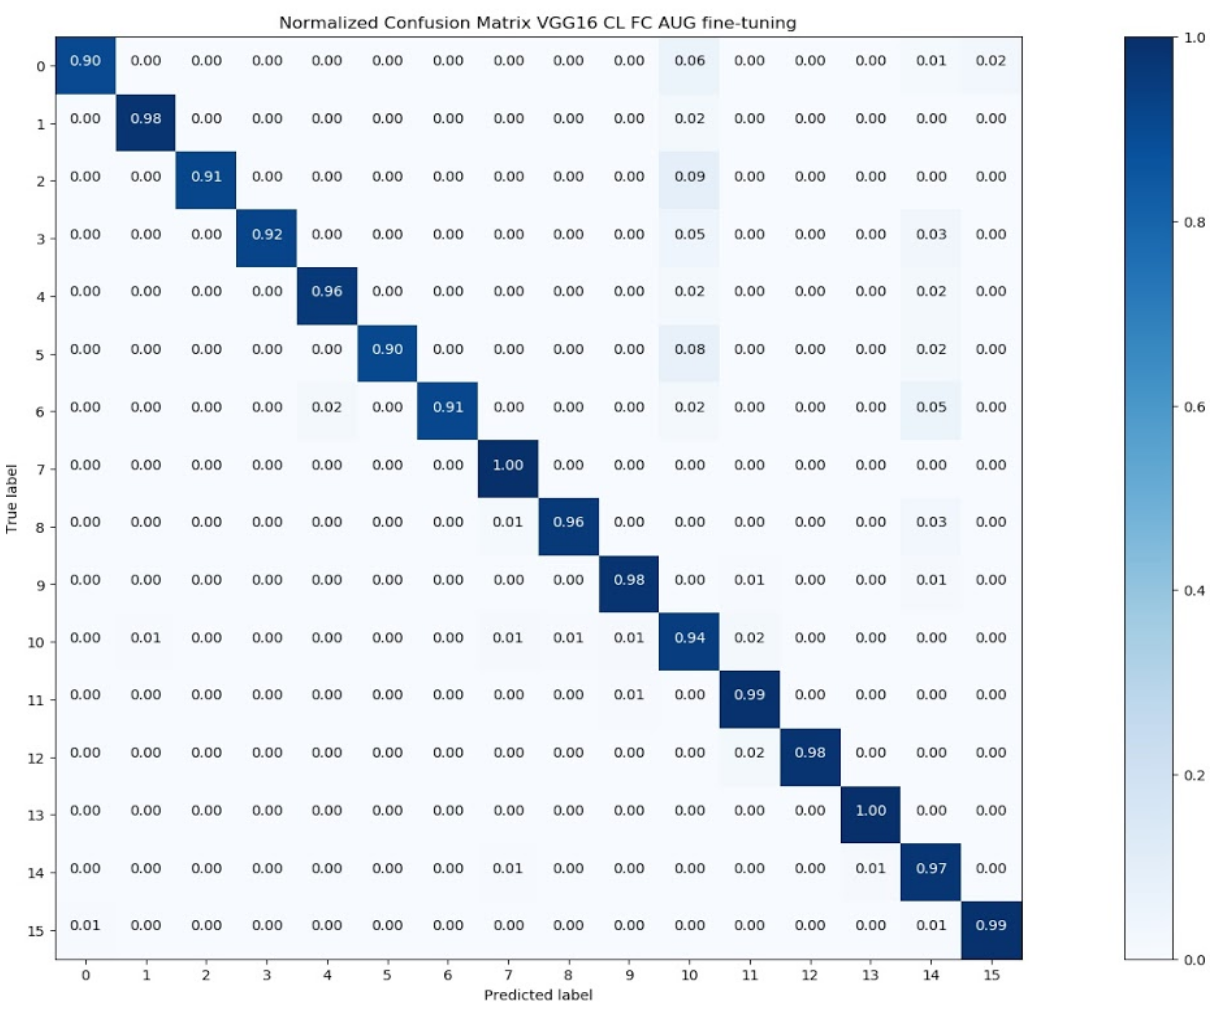
\includegraphics[scale=0.5]{image31.png}
\end{figure}

\subsection{Score F1 e Score mF1}
\begin{center}
	\begin{tabular}{| l | l | l | l |}
		\hline
		Classe & Score F1 \\ \hline
		0 & 0.94 \\ \hline
		1 & 0.97 \\ \hline
		2 & 0.95 \\ \hline
		3 & 0.95 \\ \hline
		4 & 0.97 \\ \hline
		5 & 0.94 \\ \hline
		6 & 0.95 \\ \hline
		7 & 0.95 \\ \hline
		8 & 0.96 \\ \hline
		9 & 0.98 \\ \hline
		10 & 0.92 \\ \hline
		11 & 0.97 \\ \hline
		12 & 0.99 \\ \hline
		13 & 0.99 \\ \hline
		14 & 0.97 \\ \hline
		15 & 0.99 \\ \hline 
		{\bf Score mF1} & 0.96 \\ \hline							
	\end{tabular}
\end{center}
Con questa architettura abbiamo raggiunto una {\bf accuracy} di {\bf 0.97} sul validation.

\section{Regressione}
\begin{figure}[H]
	\centering
	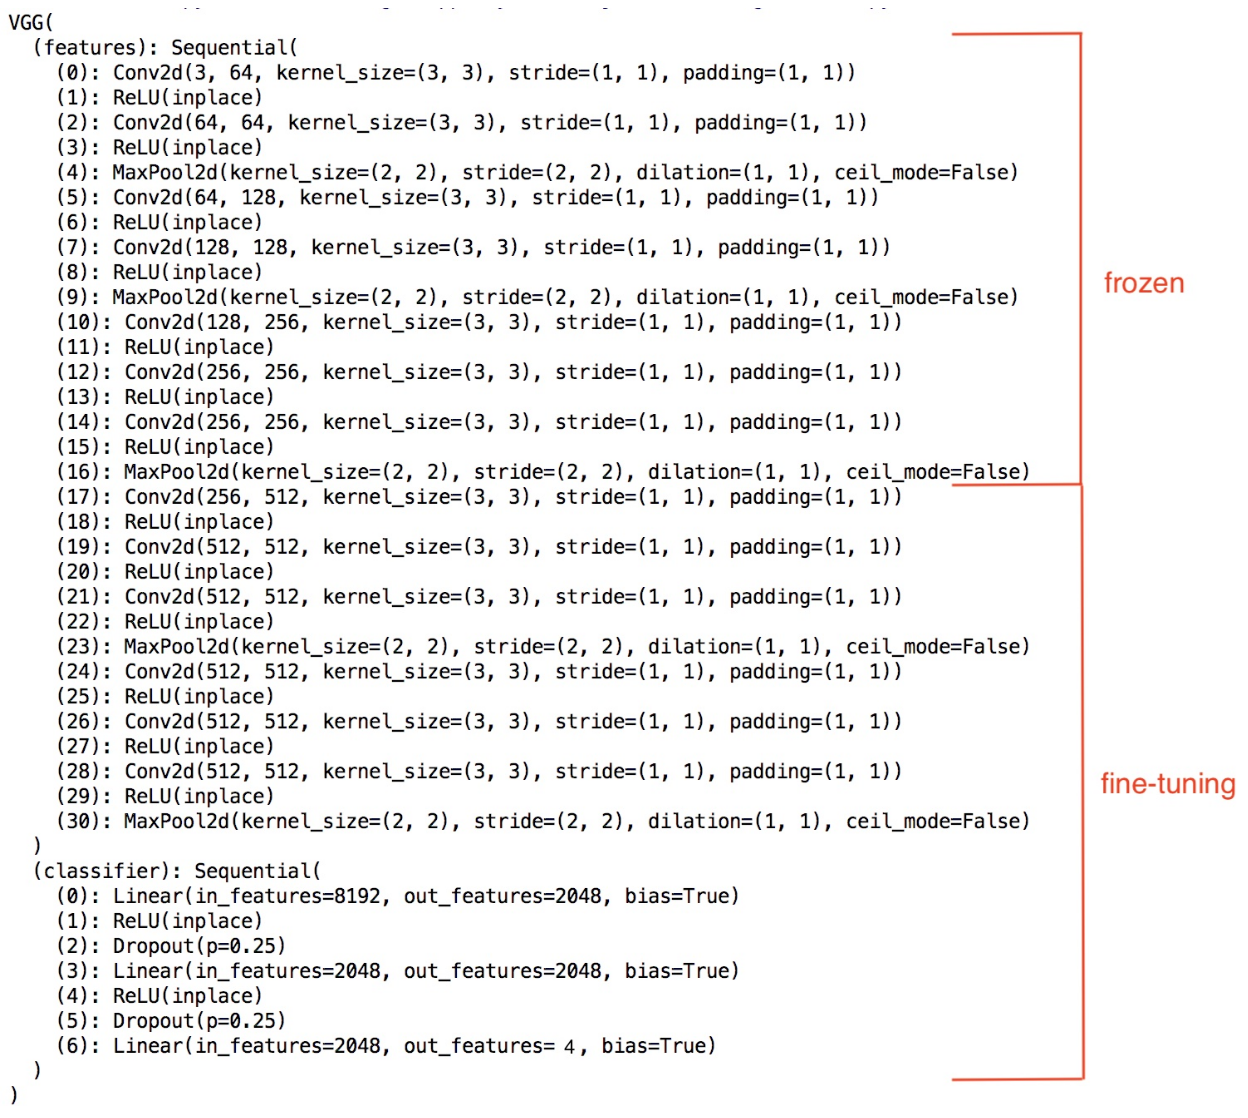
\includegraphics[scale=0.70]{image32.png}
\end{figure}
Poiché il task di regressione richiede in output 4 numeri reali x, y, u, v, sono stati modificati gli ultimi livelli lineari impostando a 4 le features di output dell’ultimo livello. \\
Per la procedura di training utilizziamo: 
\begin{itemize}
	\item[•]Learning rate: 0.00001
	\item[•]Momentum: 0.9
	\item[•]Weight decay: 0.000001
\end{itemize}
Come loss function da ottimizzare utilizziamo MSE loss, come funzione di attivazione utilizziamo ReLU, mentre come metodo di learning utilizziamo SGD. \\
Poiché abbiamo da stimare quattro numeri reali x, y, u, v, utilizziamo a tale scopo quattro loss functions, una per ogni valore, le quali verranno ottimizzate assieme durante la procedura di training. \\
Abbiamo allenato il modello per 400 epoche, ed abbiamo ottenuto i seguenti risultati:

\subsection{Loss functions}
\begin{figure}[H]
	\centering
	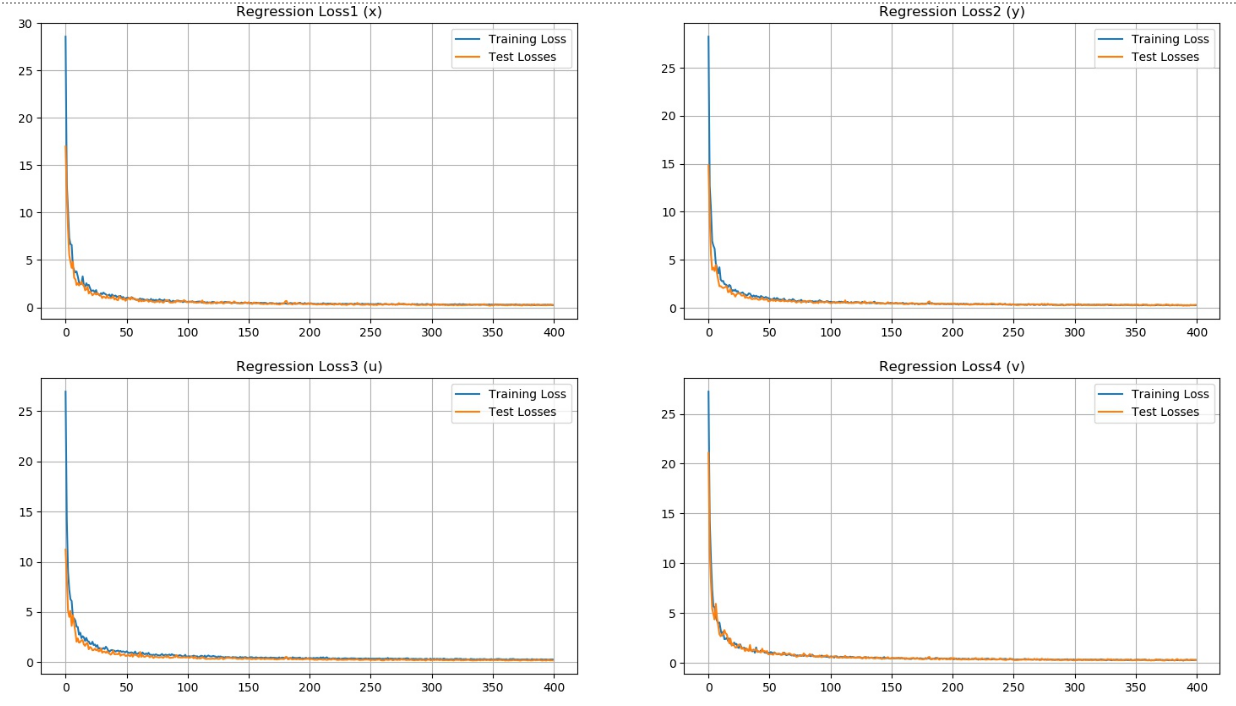
\includegraphics[scale=0.70]{image33.png}
\end{figure}
Dai 4 plot che mostrano le loss function, si può osservare come esse tendono a convergenza. A prova di ciò otteniamo valori ottimali con questa strategia.

\subsection{MSE errors}
\begin{center}
	\begin{tabular}{| l | l | l | l |}
		\hline
		MSE sul parametro X & 0.71 \\ \hline
		MSE sul parametro Y & 0.26 \\ \hline
		MSE sul parametro U & 0.05 \\ \hline
		MSE sul parametro V & 0.04 \\ \hline							
	\end{tabular}
\end{center}

\subsection{REC curves}
Le REC curve rappresentano un metodo grafico per valutare la bontà di un metodo di regressione. Inoltre, alla curva è spesso associata l'area sopra la curva (AOC) per offrire una misura dell'errore del metodo.
\begin{figure}[H]
	\centering
	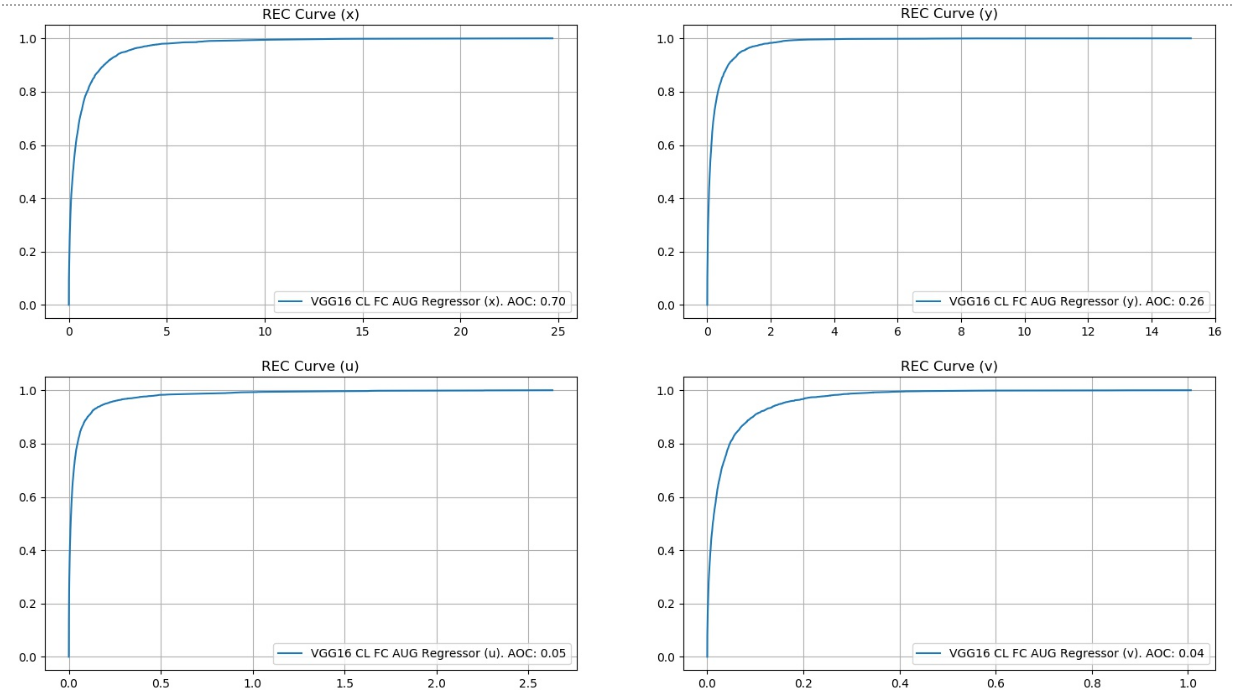
\includegraphics[scale=0.70]{image34.png}
\end{figure}

\subsubsection{RMS error}
errore RMS (Root Mean Square) medio e mediano relativo a posizione (in metri) e orientamento (in gradi):
\begin{center}
	\begin{tabular}{| l | l | l | l |}
		\hline
		Mean location error & 0.79 m \\ \hline
		Median location error & 0.65 m \\ \hline
		Mean orientation error & {9.60\textdegree} \\ \hline
		Median orientation error & {6.16\textdegree} \\ \hline							
	\end{tabular}
\end{center}